\subsection{Formato.}

Los datos proporcionados por las plataformas tienen un gran volumen, ya que como comentabamos anteriormente, se recolectan
el mayor numero de datos posibles.Este documento contara con multiples muestras para las que
se especifica un conjunto campos. Estos conjuntos de campos son similares entre ellos, pero no tienen por que ser identicos. 
De estos datos, se debera realizar una seleccion de las muestras relevantes, y de estas, los campos necesarios para representar
una informacion especifica.


A continuacion podemos ver varios ejemplos el primero de ellos esta tomado del portal de datos abiertos europeo
\footnote{\url{https://tinyurl.com/y3d76525}} y el segundo del portal de datos abiertos norte americano\footnote{\url{https://data.cityofnewyork.us/api/views/kku6-nxdu/rows.json?accessType=DOWNLOAD}}.

\begin{figure}[h]
    \centering
    \subfigure[EEUU Open Portal.Demographic Statistics By Zip Code]
     {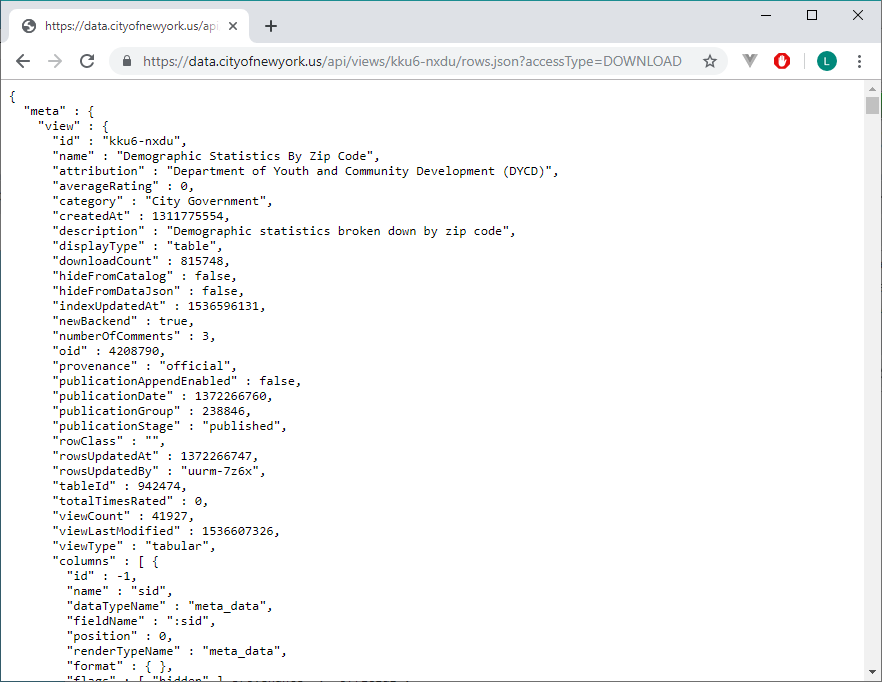
\includegraphics[width=5cm]{ExampleOpenDataEEUU}}
    \hfill
     \subfigure[European Open Portal. Air pollutant concentrations 2015]
    {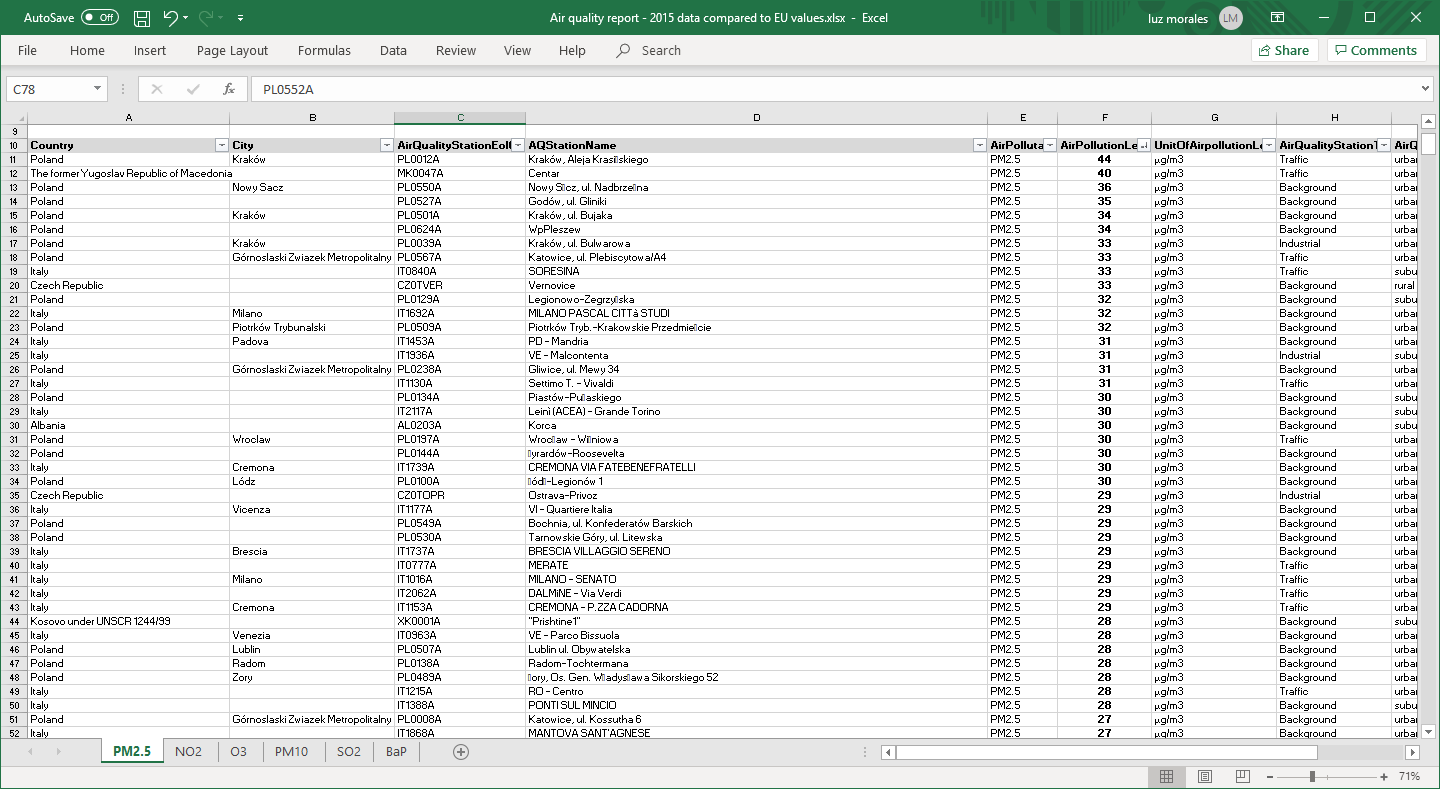
\includegraphics[width=7cm]{ExampleOpenDataEuropean}}
    \caption{Open Data Examples}
\end{figure}

    

    
\subsubsection{How to solve it} 
A traves de una serie de procesos como son  la extraccion, transformacion y 
limpieza de los datos, se obtienen los datos que se necesitan acorde a nuestro diseno. Estos procesos pueden llegar
a ser muy tediosos si no se automatizan.
Veremos estos procesos en los siguientes apartados.
\subsubsection{How we solve it. Aire Guru} 

Los datos extraidos estan en formato GeoJSON, este formato proporciona un objeto JSON con subdocumentos anidados, cada uno de estos
subdocumentos contiene un conjunto de datos en forma clave valor. 
En la siguiente figura podemos ver el principio del documento descargado el 09 de Junio del 2019 
\footnote{\url{https://datosabiertos.malaga.eu/recursos/ambiente/calidadaire/calidadaire.json}}\\
\newpage
\begin{figure}[h]
    \centering
   \subfigure[Primer subdocumento]{ \centering 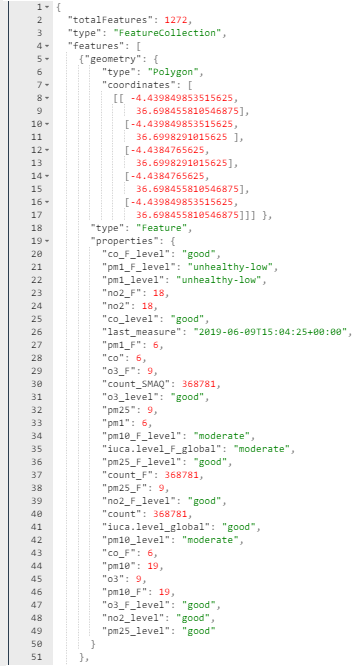
\includegraphics[width=4.75cm]{geoJsonAirQualityData1}}
   \hfill
   \subfigure[Segundo subdocumento]{ \centering 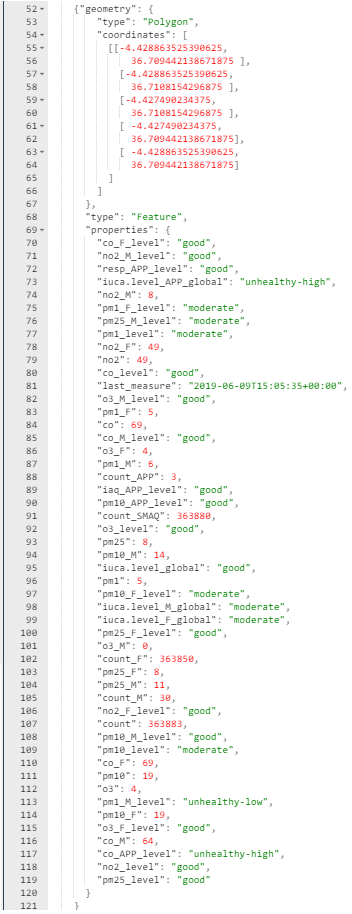
\includegraphics[width=4.75cm]{geoJsonAirQualityData2}}
 
    \caption{Air quality Document [09/06/2019].Open Data Portal Malaga}
    \end{figure}
    
En este extracto podemos ver los primeros dos subdocumentos. Cada subdocumento contiene las coordenadas de la estacion medidora de la calidad
del aire, la fecha y hora cuando se registro la medida y a continuacion los valores de las mediciones. 
En la figura siguiente podemos encontrar la descripcion proporcionada por el portal de datos abiertos.
\begin{figure}[ht]
    \centering
    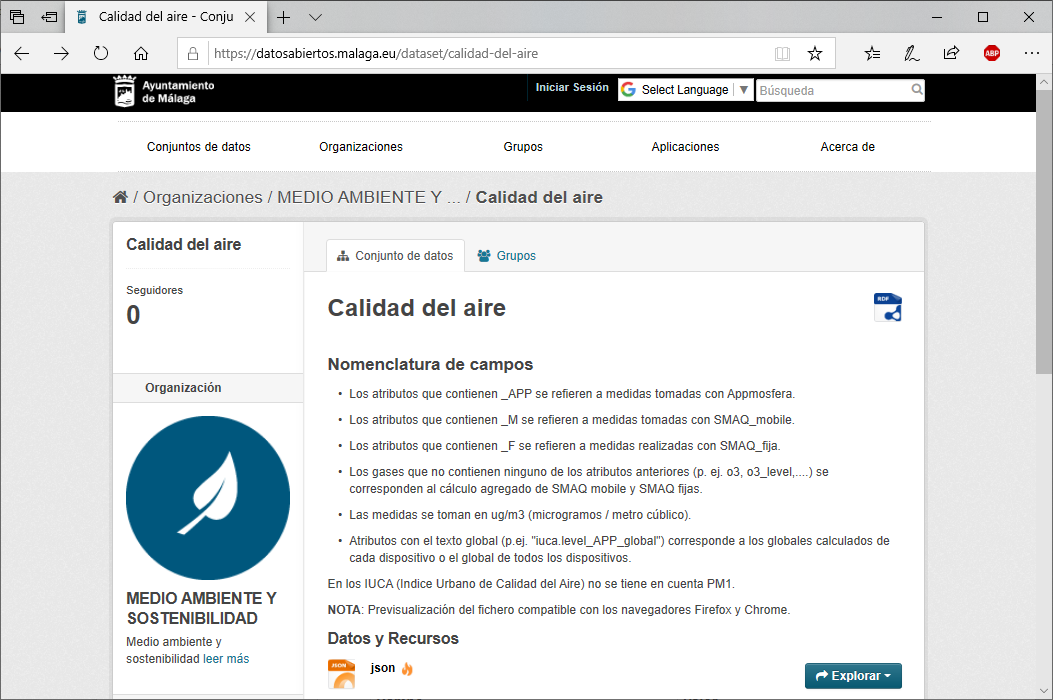
\includegraphics[width=8cm]{geoJsonAirQualityDataDescription}
    \caption{Air quality data description [09/06/2019].Open Data Portal Malaga}
\end{figure}



Para una descripcion mas en detalle de las medidas, tenemos que recurrir a un recurso externo, en este caso nos pusimos en contacto directamente con
la empresa que instala las estaciones de medida UrbanClouds \footnote{\url{https://urbanclouds.city/es/}} y proporciona los datos al ayuntamiento de Malaga.

Despues de seleccionar los campos necesarios deacurdo a nuestro diseno, se han realizado diferentes tareas de limpieza y transformacion,
como la eliminacion de datos no relevantes, por ejemplo el identificador de la estacion de medida, ya que el conjunto de datos
contiene las coordenadas de la estacion y para nosotros es mucho mas interesante.
Transformacion de campos a un formato adecuado, por ejemplo la fecha y hora en el que la medida ha sido tomada se almacena en formato fecha
en vez de cadena como se proporciona en el conjunto de datos en crudo.
Este conjunto de datos ofrece una o varias medidas por cada contaminante, que puede representarse por tres campos distintos, una medida 
cuantitativa, una cualitativa de la estacion fija de medida y una cualitativa de una estacion movil. Anadiremos un campo con la medida
mas relevante y eliminaremos las demas para minimizar el tiempo de procesado.

Por seguridad, se ha implementado una segunda arquitectura totalmente independiente que recolecta los datos y almacena en crudo.


\paragraph{Evaluation} \mbox{} 
\begin{itemize}
    \done Los datos necesarios para nuestro modelo han sido extraidos de los datos en crudo
    \done Podemos entender  que significa cada uno de los campos representados en el conjunto de dato gracias a la informacion
    complementaria presentada en el portal de datos abiertos y por la informacion proporcionada por la empresa encargada de 
    recolectar los datos.
    
\end{itemize}
\newpage
